%%%%%%%%%%%%%%%%%%%%%%%%%%%%%%%%%%%%%%%%%
% Beamer Presentation
% LaTeX Template
% Version 1.0 (10/11/12)
%
% This template has been downloaded from:
% http://www.LaTeXTemplates.com
%
% License:
% CC BY-NC-SA 3.0 (http://creativecommons.org/licenses/by-nc-sa/3.0/)
%
%%%%%%%%%%%%%%%%%%%%%%%%%%%%%%%%%%%%%%%%%

%----------------------------------------------------------------------------------------
%	PACKAGES AND THEMES
%----------------------------------------------------------------------------------------

\documentclass{beamer}

\mode<presentation> {

% The Beamer class comes with a number of default slide themes
% which change the colors and layouts of slides. Below this is a list
% of all the themes, uncomment each in turn to see what they look like.

\usetheme{default}
%\usetheme{AnnArbor}
%\usetheme{Antibes}
%\usetheme{Bergen}
%\usetheme{Berkeley}
%\usetheme{Berlin}
%\usetheme{Boadilla}
%\usetheme{CambridgeUS}
%\usetheme{Copenhagen}
%\usetheme{Darmstadt}
%\usetheme{Dresden}
%\usetheme{Frankfurt}
%\usetheme{Goettingen}
%\usetheme{Hannover}
%\usetheme{Ilmenau}
%\usetheme{JuanLesPins}
%\usetheme{Luebeck}
%\usetheme{Madrid}
%\usetheme{Malmoe}
%\usetheme{Marburg}
%\usetheme{Montpellier}
%\usetheme{PaloAlto}
%\usetheme{Pittsburgh}
%\usetheme{Rochester}
%\usetheme{Singapore}
%\usetheme{Szeged}
%\usetheme{Warsaw}

% As well as themes, the Beamer class has a number of color themes
% for any slide theme. Uncomment each of these in turn to see how it
% changes the colors of your current slide theme.

%\usecolortheme{albatross}
%\usecolortheme{beaver}
%\usecolortheme{beetle}
%\usecolortheme{crane}
%\usecolortheme{dolphin}
%\usecolortheme{dove}
%\usecolortheme{fly}
%\usecolortheme{lily}
%\usecolortheme{orchid}
%\usecolortheme{rose}
%\usecolortheme{seagull}
%\usecolortheme{seahorse}
%\usecolortheme{whale}
%\usecolortheme{wolverine}

%\setbeamertemplate{footline} % To remove the footer line in all slides uncomment this line
%\setbeamertemplate{footline}[page number] % To replace the footer line in all slides with a simple slide count uncomment this line

%\setbeamertemplate{navigation symbols}{} % To remove the navigation symbols from the bottom of all slides uncomment this line
}
\usepackage{bbm}
\usepackage{graphicx} % Allows including images
\usepackage{booktabs} % Allows the use of \toprule, \midrule and \bottomrule in tables

%----------------------------------------------------------------------------------------
%	TITLE PAGE
%----------------------------------------------------------------------------------------

\title[Short title]{Generalized estimating equation modeling on correlated microbiome sequencing data with longitudinal measures } % The short title appears at the bottom of every slide, the full title is only on the title page

\author{Emily Palmer} % Your name
\institute[OSU] % Your institution as it will appear on the bottom of every slide, may be shorthand to save space
{
Journal Club, Oregon State University  %\\ % Your institution for the title page
%\medskip
%\textit{john@smith.com} % Your email address
}
\date{\today} % Date, can be changed to a custom date

\begin{document}

\begin{frame}
\titlepage % Print the title page as the first slide
\end{frame}

\begin{frame}
\frametitle{Overview} % Table of contents slide, comment this block out to remove it
\tableofcontents % Throughout your presentation, if you choose to use \section{} and \subsection{} commands, these will automatically be printed on this slide as an overview of your presentation
\end{frame}

%----------------------------------------------------------------------------------------
%	PRESENTATION SLIDES
%----------------------------------------------------------------------------------------

%------------------------------------------------
\section{Introduction} % Sections can be created in order to organize your presentation into discrete blocks, all sections and subsections are automatically printed in the table of contents as an overview of the talk
%------------------------------------------------

%\subsection{Subsection Example} % A subsection can be created just before a set of slides with a common theme to further break down your presentation into chunks

\begin{frame}[t]{Introduction}
  Challenges of applying regression models on association studies of microbiome composition and environmental factors
  \begin{itemize}
    \item Many OTUs, potentially correlated
    \item Repeated Measures (longitudinal, other repeated measures)
    \item OTU data has excessive zeros
  \end{itemize}
\end{frame}
%--- Next Frame ---%



\begin{frame}
\frametitle{Goals}
\begin{itemize}
  \item Estimate correlations between multiple OTUs
  \item Incorporate correlations into models with longitudinal OTU measures
  \item Estimate predictors effects using GEEs
  \item Two-part Microbiome Taxonomic Longitudinal Correlation (MLTC) model
\end{itemize}
\end{frame}



\begin{frame}[t]{Correlation matrix of taxonomic structure - Assumptions}
  \begin{itemize}
    \item Assume that OTUs that belong to the same taxa at some higher level have some correlation
    \item All OTUs will belong to same taxa at highest level, so there are $\binom{N}{2}$ possible correlations - infeasible to model
    \item Assume that two pairs of OTUs have the same correlation if the first common taxa of both pairs are identical


  \end{itemize}
\end{frame}
%--- Next Frame ---%


\begin{frame}
\frametitle{Example}

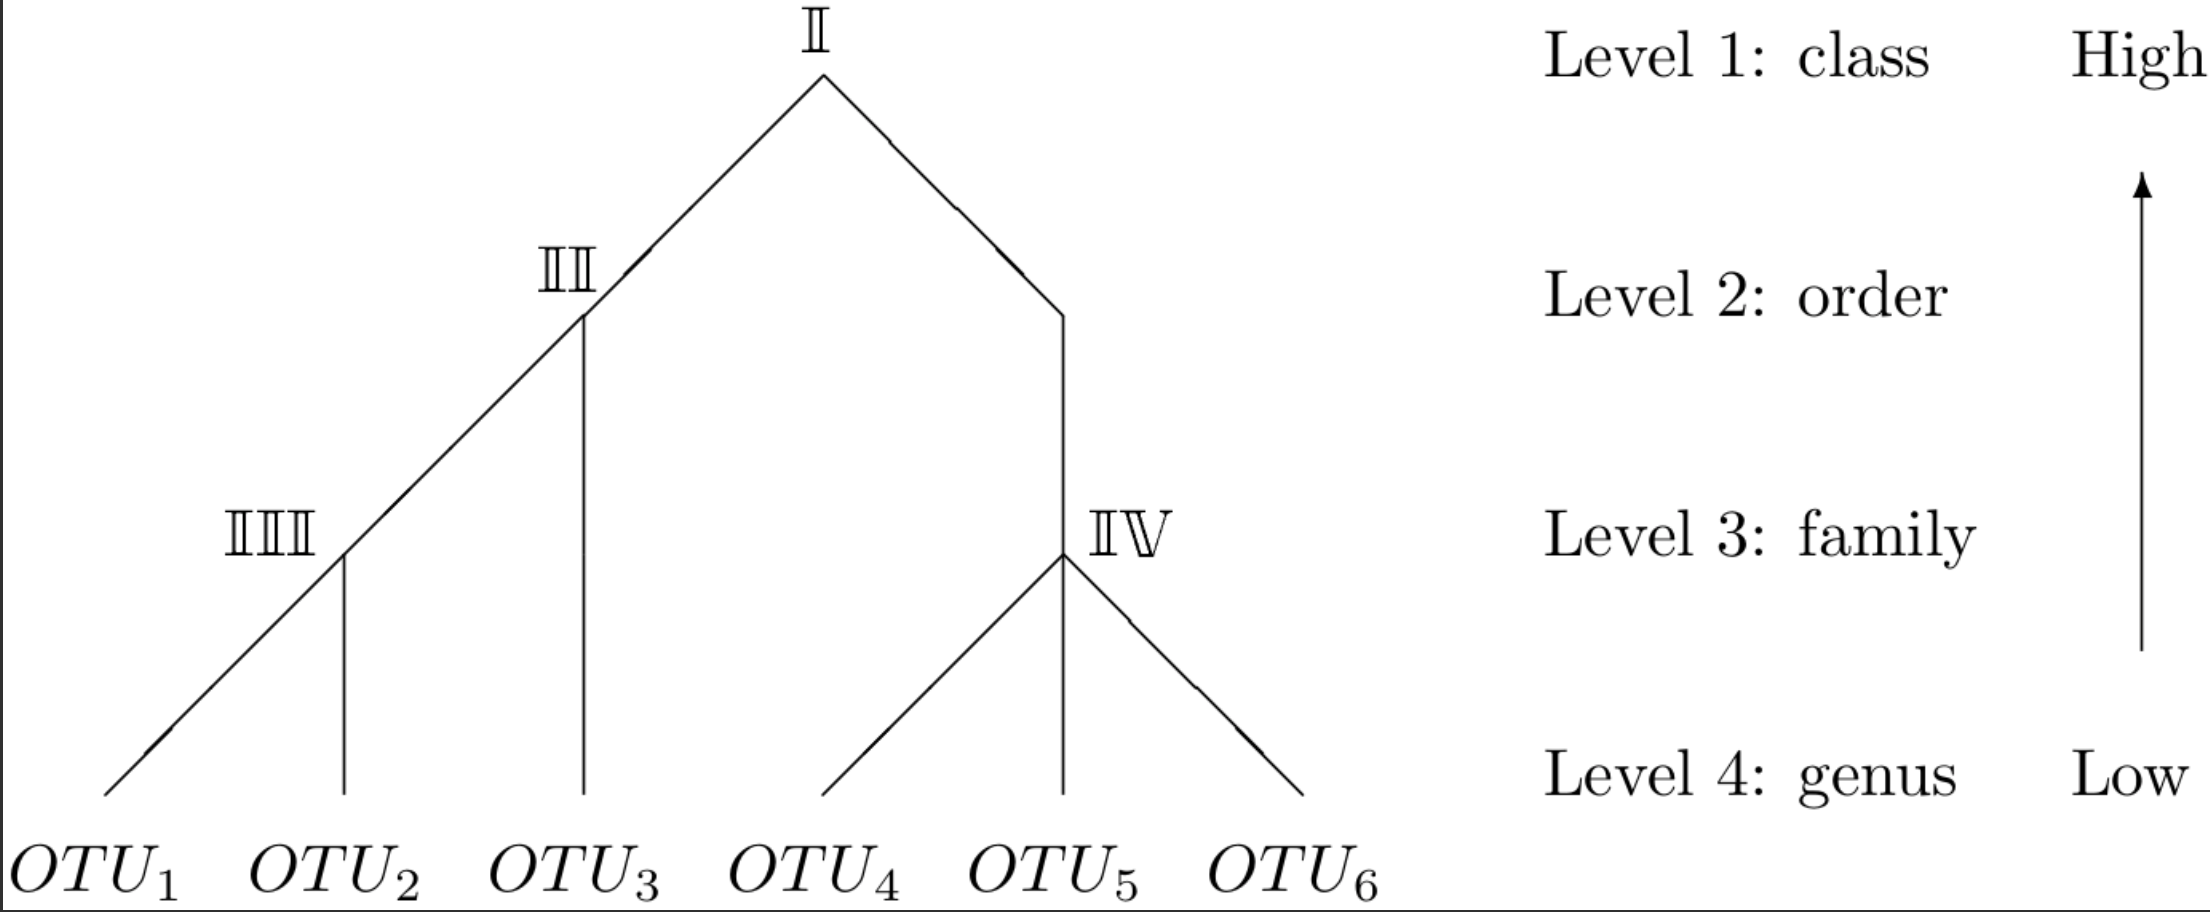
\includegraphics[width = \textwidth]{otu_tree.png}

\end{frame}

\section{Correlation structure}
\subsection{Taxonomic correlation structure of OTUs}

\begin{frame}[t]{Notation and Definitions}
  \begin{itemize}
    \item $I$ levels:
    \begin{itemize}
      \item 1st taxonomic level is the level at which all observed $N$ OTUs belong to the same taxon but not at one level lower
    \end{itemize}
    \item $M_i$: number of taxa at level $i$ ($M_1 = 1, M_I = N$)
    \item $t_{m_i, i}$: taxon at level $i$ for $m_i = 1, \ldots , M_i$
    \item $n_{m_i, i}$: number of OTUs belonging to taxon $t_{m_i,i}$. $\mathbf{n}_i = (n_{1i}, \ldots , n_{M_i,i})$
%    \item If $\mathcal{P}^*$ and $\mathcal{P}^\dagger$ are two pairs of OTUs, with correlation $\rho^*$ and $\rho^\dagger$. $t_{m_i^*, i^*}$ is first common taxa of $\mathcal{P}^*$ $t_{m_i^\dagger, i^\dagger}$ is first common taxa of $\mathcal{P}^\dagger$

%    $$\rho^* = \rho^\dagger \leftrightarrow t_{m_i^*, i^*} = t_{m_i^\dagger, i^\dagger}$$
  \end{itemize}
\end{frame}
%--- Next Frame ---%


%--- Next Frame ---%


\begin{frame}
\frametitle{Example}

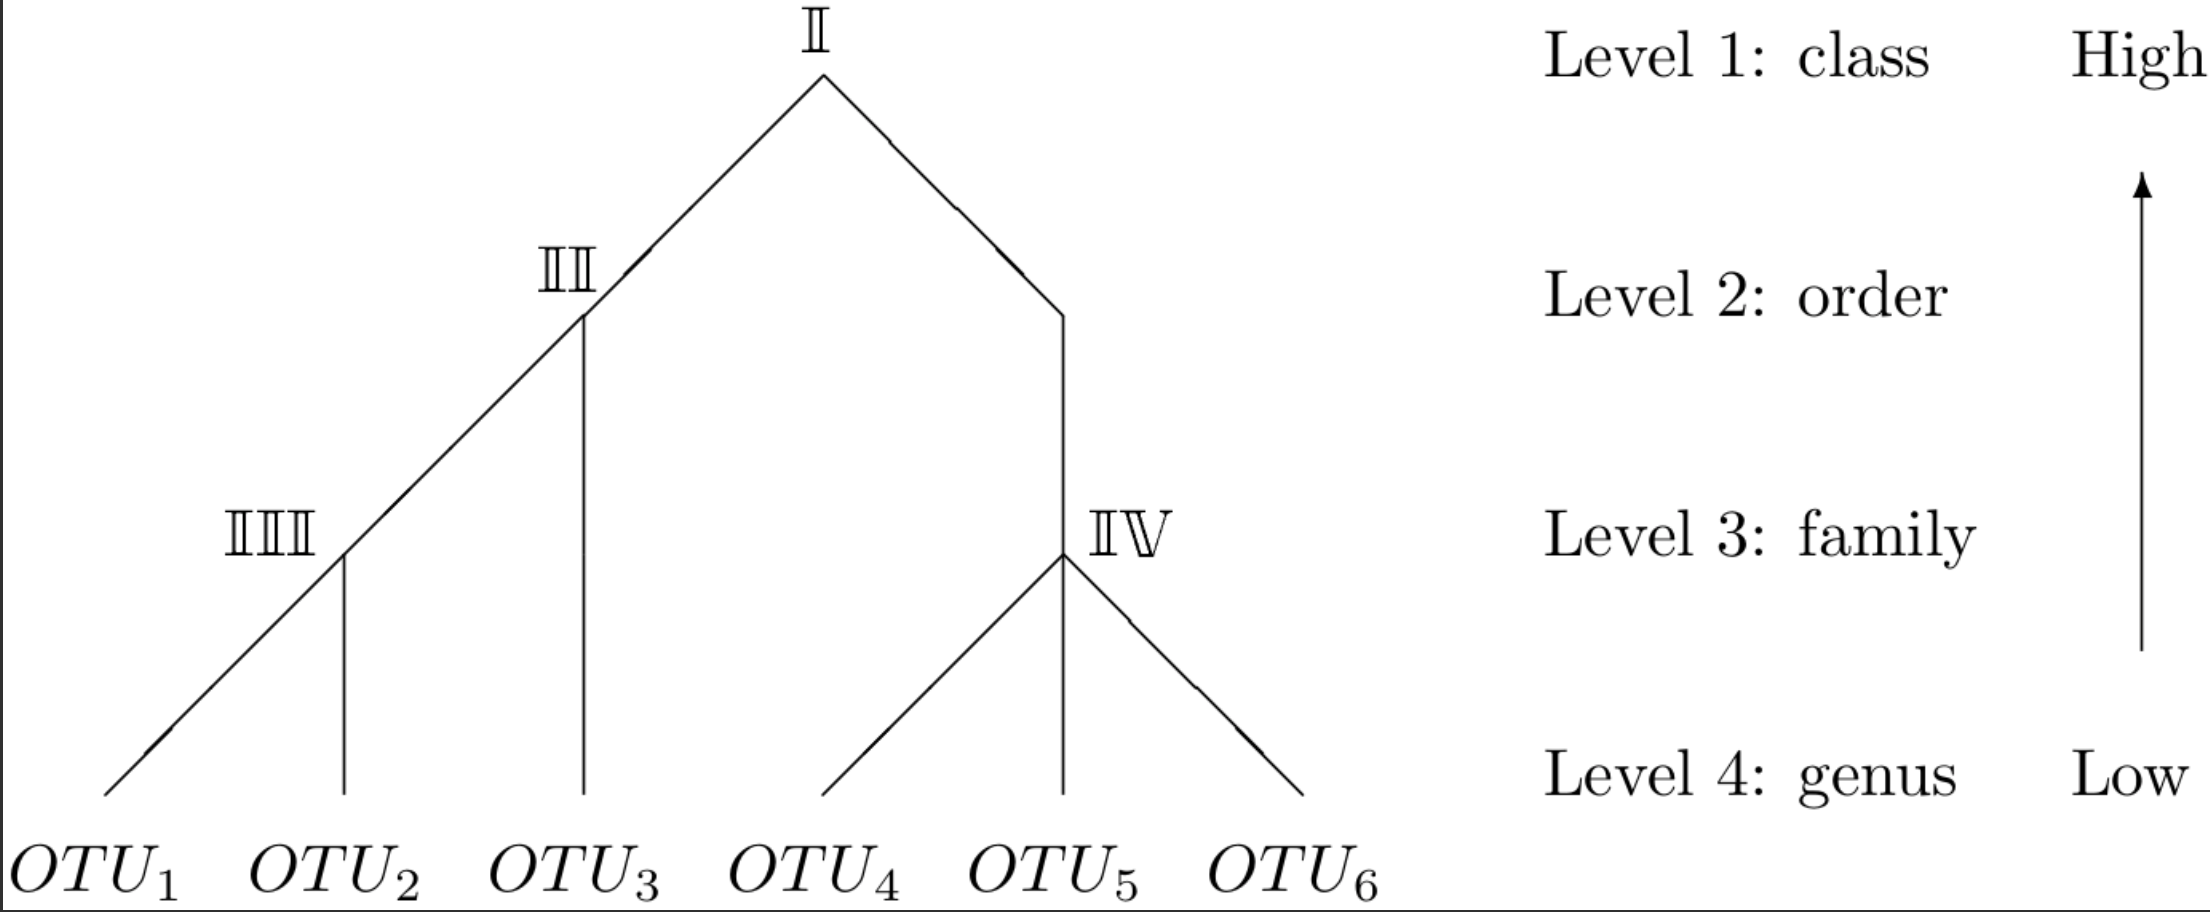
\includegraphics[width = \textwidth]{otu_tree.png}

$M_1 = 1, M_2 = 2, M_3 = 3, M_4 = 6$, $\boldsymbol n_1 = 6, \boldsymbol n_2 = (3,3), \boldsymbol n_3 = (2,1,3), \boldsymbol n_4 = (1,1,1,1,1,1)$

$\mathbb{I}$ represents correlation of same class different orders,\\ $\mathbb{II}$ correlation of same order different families,\\
$\mathbb{III}$, $\mathbb{IV}$ same family

\end{frame}

%------------------------------------------------


\begin{frame}[t]{The taxonomic structure matrix $\Gamma$}
  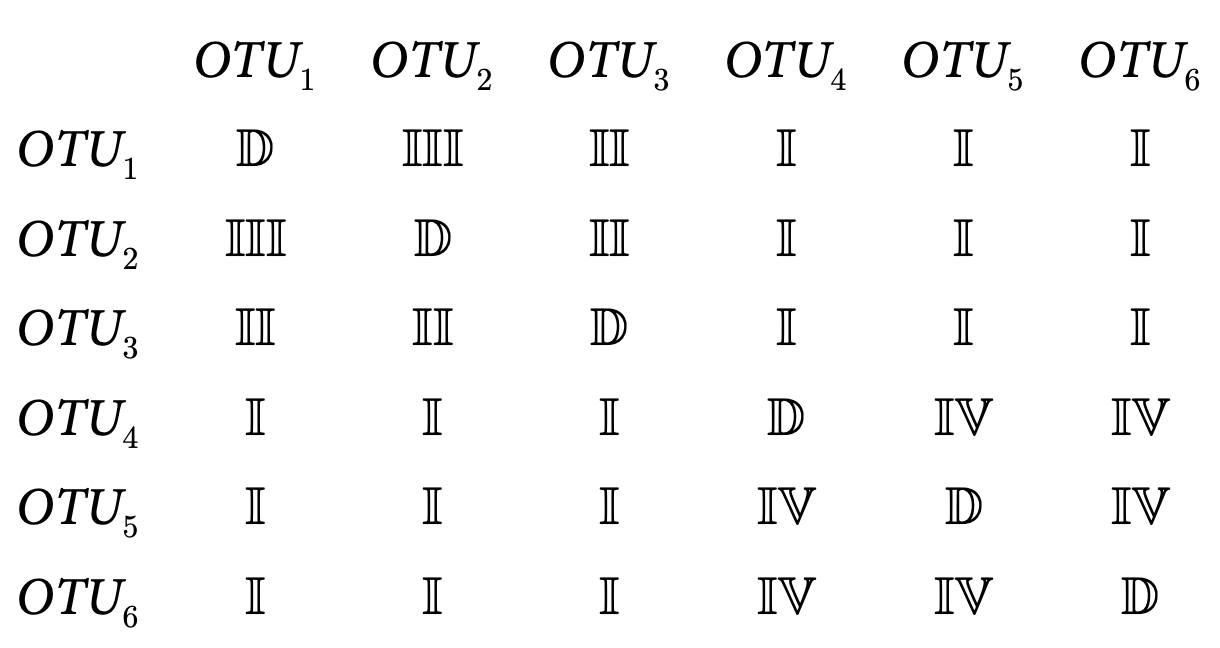
\includegraphics[width = \textwidth]{Gamma.png}
\end{frame}
%--- Next Frame ---%




\begin{frame}[t]{Finding the taxonomic structure matrix}
  \begin{itemize}
    \item Create $I-1$ $N\times N$ block matrices
    $$\boldsymbol\Gamma_i = \begin{pmatrix}
          \boldsymbol B_{1i} & & \\
          & \ddots & \\
          & & \boldsymbol B_{M_i,i}
    \end{pmatrix}$$
    For $m_i = 1, \ldots , M_i$, each block $\boldsymbol B_{1,i}$ is an $n_{m_i,i} \times n_{m_i,i}$ matrix, with diagonal entries $\mathbb{D}$ and off diagonal entries $\sum_{h=0}^{i-1}M_h + m_i$
    \item Create interim correlation after replacement at level $i$ ($\boldsymbol\Gamma^{(i)}$)
    \begin{itemize}
      \item For $i = 1$, $\boldsymbol\Gamma^{(1)} = \boldsymbol\Gamma_1$
      \item For $i = 2, \ldots , I-1$, Replace the block diagonal entries of $\boldsymbol\Gamma^{(i-1)}$ with $\boldsymbol B_{m_i,i}$, but keep all other entries the same.
    \end{itemize}
    \item Sort all elements from largest to smallest. Different ranks are the distinct correlations to estimate
  \end{itemize}
\end{frame}
%--- Next Frame ---%


  \begin{frame}
  \frametitle{Example }
  \begin{columns}[c] % The "c" option specifies centered vertical alignment while the "t" option is used for top vertical alignment
  \column{.5\textwidth} % Left column and width
  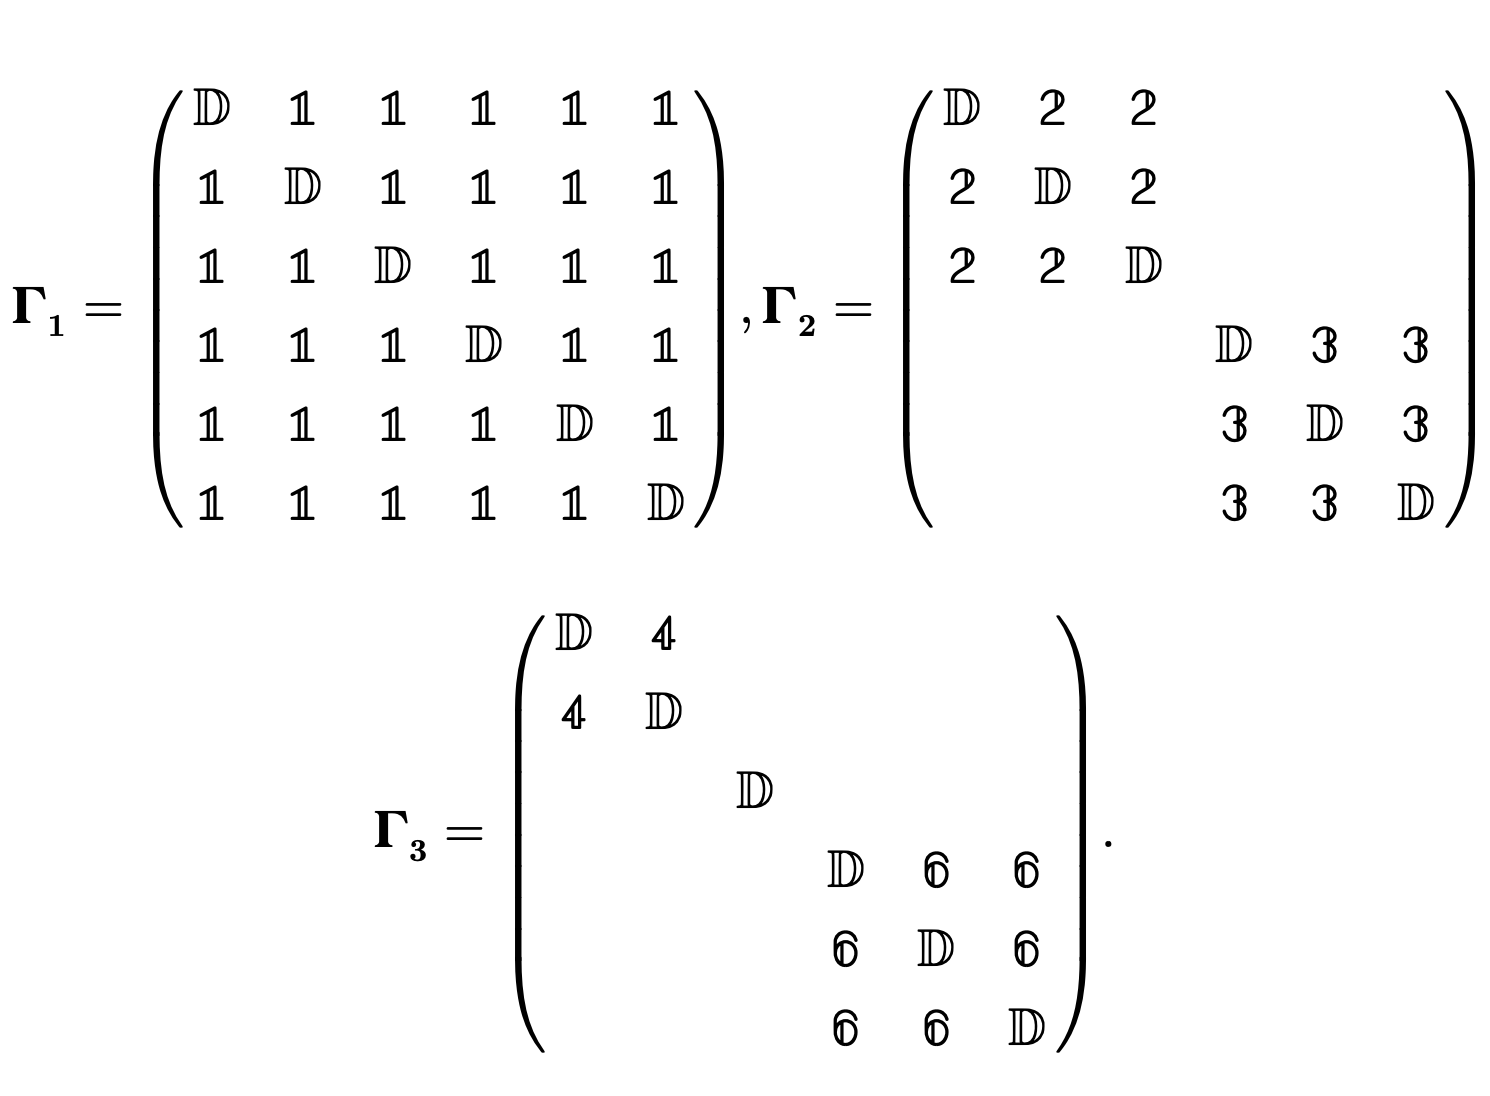
\includegraphics[width = \textwidth]{blockmatrices.png}


  \column{.5\textwidth} % Right column and width
  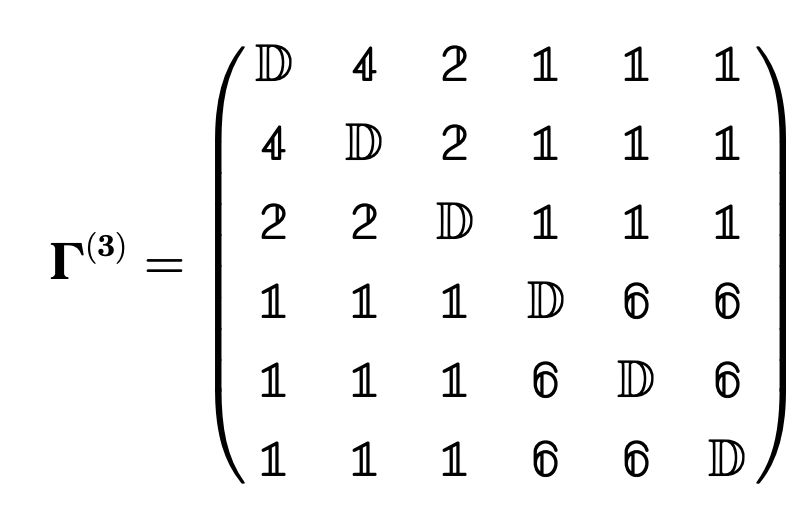
\includegraphics[width = \textwidth]{gamma3.png}
  \end{columns}

  $\boldsymbol\Gamma$ can be represented by $(\boldsymbol n_1, \ldots , \boldsymbol n_I)$
  \end{frame}

%--- Next Frame ---%
\begin{frame}[t]{The taxonomic structure matrix $\Gamma$}
  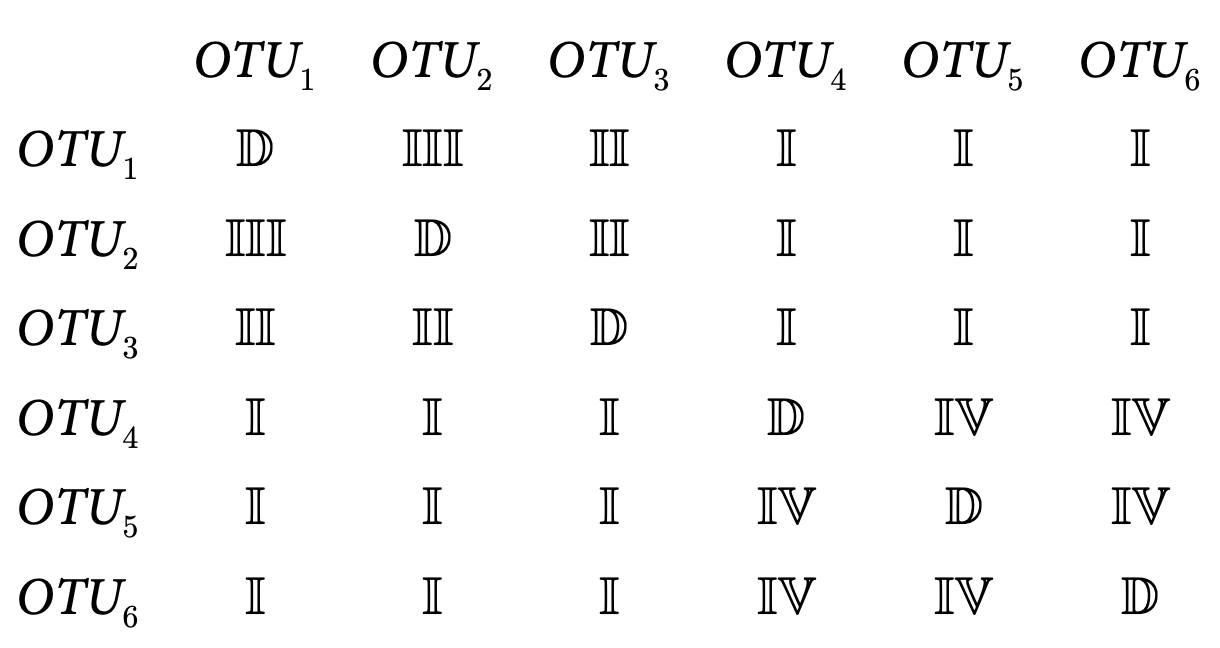
\includegraphics[width = \textwidth]{Gamma.png}
\end{frame}

\subsection{Correlation structure from longitudinal repeated measures}

\begin{frame}
\frametitle{Correlation structure from longitudinal repeated measures}

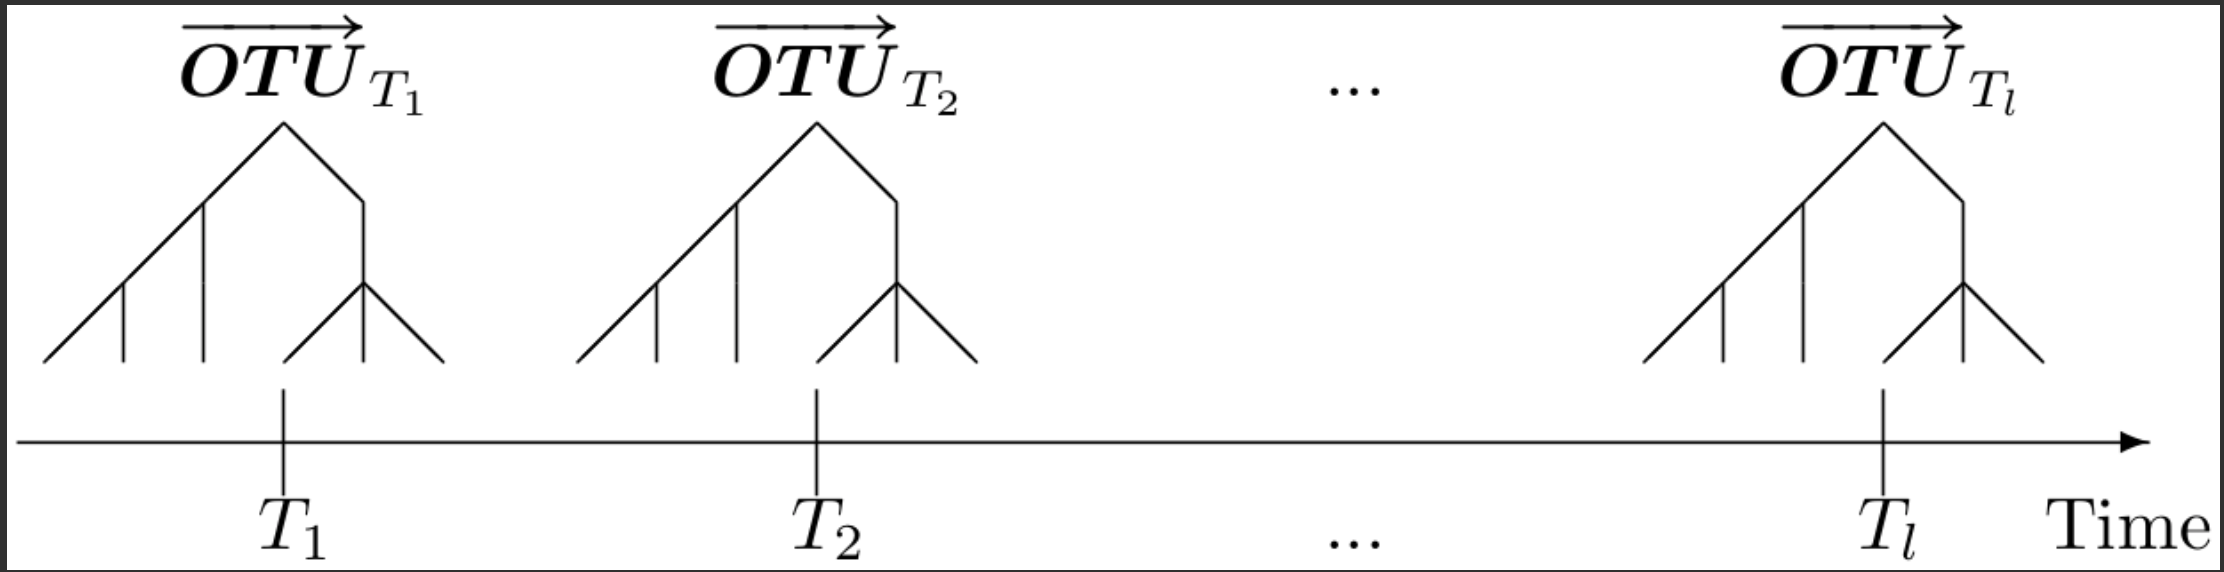
\includegraphics[width = \textwidth]{otu_time_tree.png}

\end{frame}


\begin{frame}[t]{Types of correlations between pairs of time points}

  \begin{itemize}
    \item Exchangeable
    \begin{itemize}
      \item Assumes all correlations are equal to each other
    \end{itemize}
    \item Toeplitz
    \begin{itemize}
      \item Assumes time points with equal temporal distance have equal correlation
    \end{itemize}
    \item Unstructured
    \begin{itemize}
      \item Assumes each pair has a different correlations
      \item Most complicated structure for correlation parameter estimation
    \end{itemize}
  \end{itemize}
  Correlation structure matrix for the the same individual is denoted $\Omega_T$
\end{frame}
%--- Next Frame ---%




\begin{frame}
\frametitle{Example Correlation Matrices for 3 timepoints}

\begin{columns}[c] % The "c" option specifies centered vertical alignment while the "t" option is used for top vertical alignment

\column{.45\textwidth} % Left column and width
\textbf{Exchangable structure}
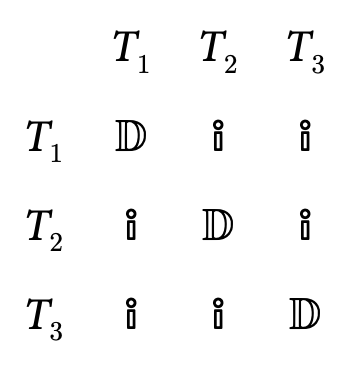
\includegraphics[width = \textwidth]{exchangeable.png}


\column{.5\textwidth} % Right column and width
\textbf{Toeplitz structure}
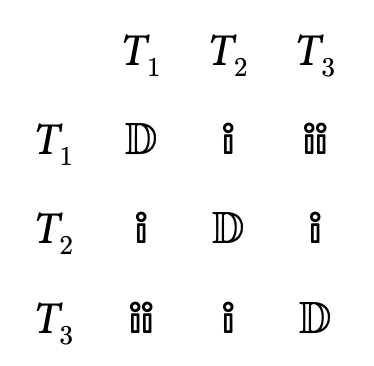
\includegraphics[width = \textwidth]{toeplitz.png}

\end{columns}
\end{frame}


\begin{frame}[t]{Combining longitudinal and sample correlation}

When both longitudinal and sample correlations exist, the repeated measure correlation matrix is all combinations of time points and repeated samples

  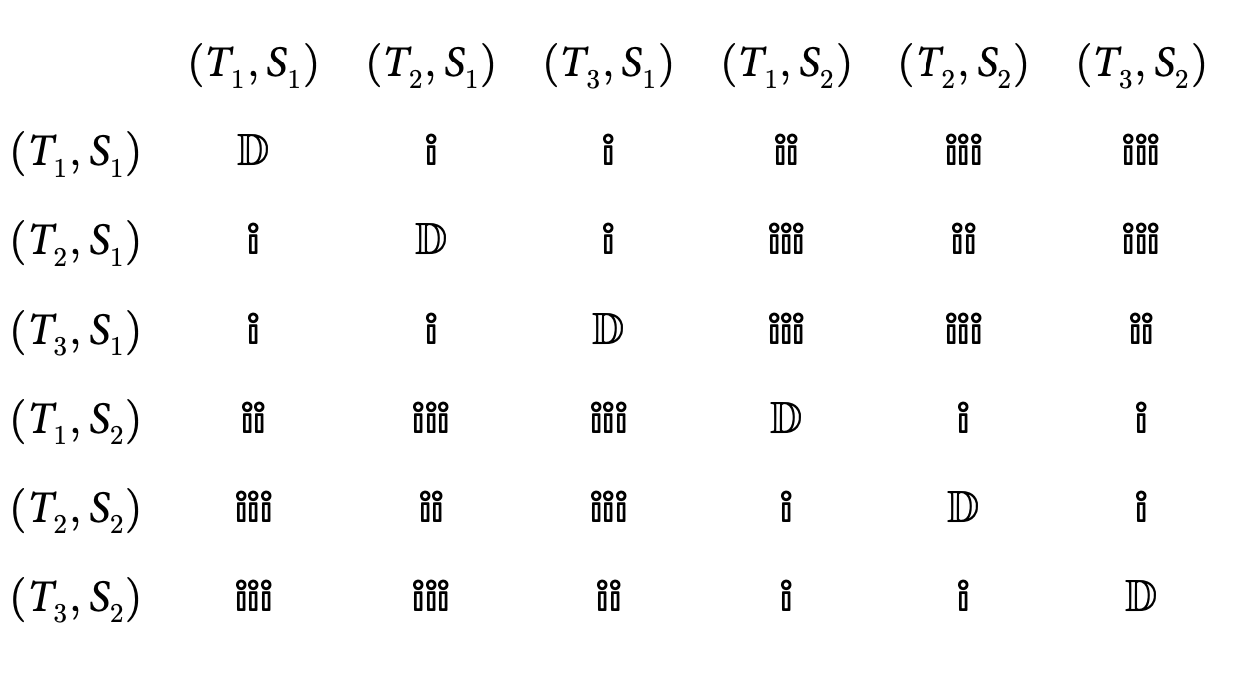
\includegraphics[width = \textwidth]{longitudinal_sample.png}

\end{frame}




\subsection{Integrative Correlation Matrix}


\begin{frame}[t]{Incorporating taxonomic structure with repeated measures}
  $\boldsymbol\Omega$ with dimension $L$, for $a,b = 1, \ldots , N$,

%$$\boldsymbol\Omega^{\boldsymbol{ab}} = \boldsymbol\Omega(\boldsymbol\Gamma_{ab}) = \begin{pmatrix}
%      \rho_{(\Gamma_{ab,\Omega_{11}})} & \cdots & \rho_{(\Gamma_{ab,\Omega_{1L}})} \\
%      \vdots & \ddots & \vdots \\
%      \rho_{(\Gamma_{ab,\Omega_{L1}})} & \cdots & \rho_{(\Gamma_{ab,\Omega_{LL}})}
%\end{pmatrix}$$
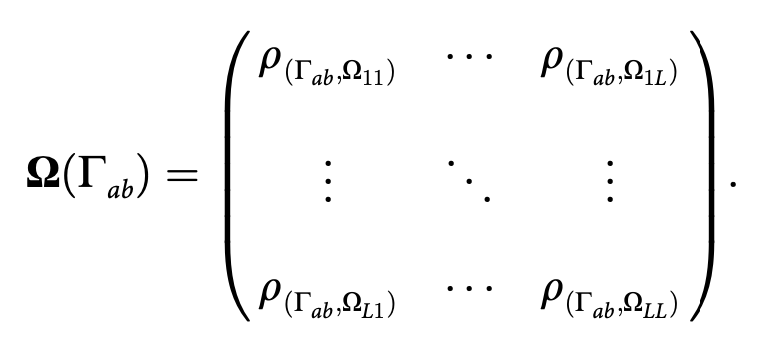
\includegraphics[width = .5\textwidth]{omega_gamma.png} 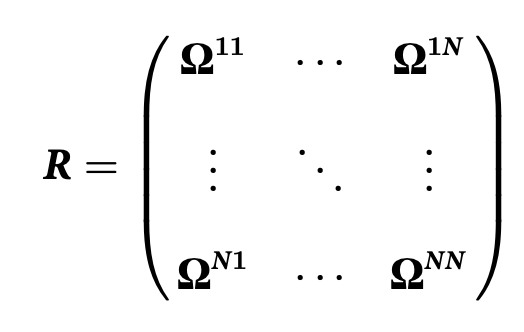
\includegraphics[width = .5\textwidth]{R.png}

Dimension of $R = (N \times L) \times (N \times L)$

Diagonals of $R = \rho(\mathbb{D},\mathbb{D})$ are 1, off-diagonals need to be estimated
\end{frame}
%--- Next Frame ---%


\begin{frame}[t]{Example R}
  For two correlated OTUs and two repeated measures at different time points

  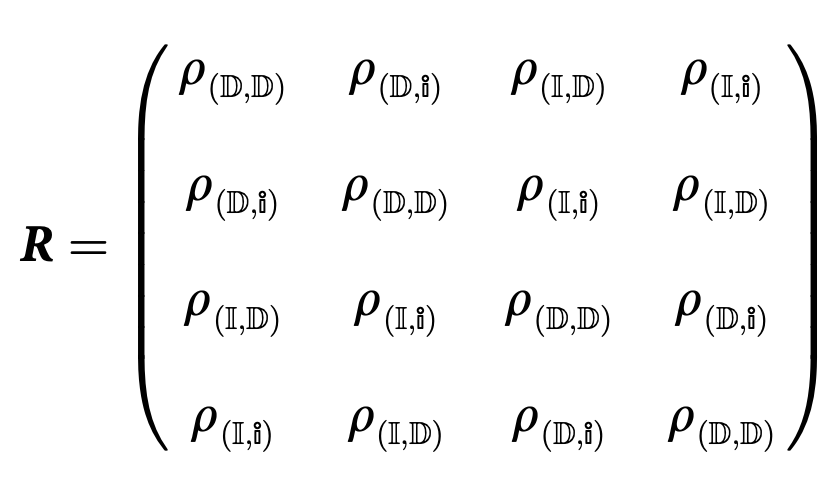
\includegraphics[width = .5\textwidth]{r_ex.png}

  \begin{itemize}
    \item $\rho_{(\mathbb{D},\mathbb{D})} = 1$
    \item $\rho_{(\mathbb{D},\mathbbm{i})}, \rho_{(\mathbb{I},\mathbb{D})}$ correlation between two time points and two OTUs
    \item $\rho_{(\mathbb{I},\mathbbm{i})}$ correlation from different OTU and different time points
  \end{itemize}
\end{frame}
%--- Next Frame ---%



\section{Microbiome Taxonomic Longitudinal Correlation model}


\begin{frame}[t]{Introduction to MTLC:}
  MTLC:
  \begin{itemize}
    \item Estimate predictor effects
    \item Estimate correlation coefficients between OTUs, longitudinal measures and other repeated measures
    \item Perform hypothesis testing of predictor effects
  \end{itemize}
\end{frame}

\subsection{General GEE framework}

\begin{frame}[t]{Generalized estimating equation framework}
  \begin{itemize}
    \item $\boldsymbol y_k = (y_{k1}, \ldots , y_{kJ_k})$ clusters, length $J_k$ for $k = 1, \ldots , K$
    \item $\mathbf{x}_{kj}$ the vector of covariates with length $p$, $j = 1, \ldots , J_k$
    \item $\boldsymbol\mu_k = (\mu_{k1}, \ldots , \mu_{kJ_k})$ mean of $\boldsymbol y_k$
    \item Each observation $y_{kj}$
    $$g(\mu_{kj}) = \mathbf{x}_{kj}'\boldsymbol\beta$$
    \item Conditional variance of $y_{kj}$
    $$\text{Var}(y_{kj}|\boldsymbol{x}_{kj}) = v(\boldsymbol \mu_{kj})\phi$$
    $v$ is the variance function depending on the distribution of $y_{kj}$, $\phi$ is dispersion parameter
  \end{itemize}
%--- Next Frame ---%
\end{frame}


\begin{frame}[t]{cont.}
  \begin{itemize}
    \item Estimate $\boldsymbol\beta$ by solving the generalized estimating equation
    $$U(\boldsymbol\beta) = \sum_{k = 1}^K \boldsymbol{D}_k'\boldsymbol{V}_{k}^{-1}(\boldsymbol{y}_k - \boldsymbol{\mu}_k) = 0$$
    \item $\boldsymbol{D}_k = \frac{d \boldsymbol\mu_k}{d \boldsymbol\beta}$, $\boldsymbol{V}_k = \boldsymbol{A}_k^{1/2}\boldsymbol{R}_k(\boldsymbol\rho)\boldsymbol{A}_k^{1/2}$,
    \item  $\boldsymbol{A}_k = diag(\mu_{k1}\phi, \ldots , \mu_{kJ_k}\phi)$ $\boldsymbol\rho$ collection of all correlation coefficients in $\boldsymbol{R_k}$
    \item $\boldsymbol R_k(\boldsymbol\rho)$ is the working correlation matrix following correlation structure $R$

  \end{itemize}
\end{frame}

\begin{frame}[t]{cont.}
  \begin{itemize}
    \item $\phi, \boldsymbol\rho$ also need to be estimated
    $$\hat\phi = \frac{1}{\sum_{k=1}^K J_k - p}\sum_{k=1}^K\sum_{j=1}^{J_k} e^2_{kj}$$
    where $e_{kj}$ is the Pearson residual
    \item $\hat{\boldsymbol\rho}$ is estimated as a function of $\phi$ and $e_{kj}$, depending on the correlation structure $R $
    \item Iterative - switch between estimating $\boldsymbol\beta$ from fixed value of $\hat\phi$ and $\hat{\boldsymbol\beta}$ and estimating $\phi$ and $\boldsymbol\rho$ for a fixed value of $\hat{\boldsymbol\beta}$
  \end{itemize}
\end{frame}
%--- Next Frame ---%

%--- Next Frame ---%

\begin{frame}[t]{Hypothesis testing}

  \begin{itemize}
    \item From GEE theory $\hat{\boldsymbol \beta}$ is asymptotically normally distributed with mean $\boldsymbol \beta$ and variance\\
    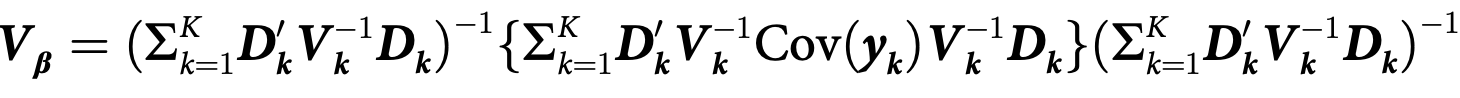
\includegraphics[width = \textwidth]{beta_var.png}
    \item Wald test statistic for testing $H_0: \boldsymbol{C\beta} = \boldsymbol c$
    $$\boldsymbol W = (\boldsymbol C \hat{\boldsymbol\beta} - \boldsymbol c)'(\boldsymbol C \hat{\boldsymbol V}_\beta \boldsymbol C')^{-1}(\boldsymbol C \hat{\boldsymbol\beta} - \boldsymbol c)$$
    \item $W \overset{d}{\to} \chi^2_{(q)}$ where $q$ is the rank of $\boldsymbol{C}$

  \end{itemize}

\end{frame}

%--- Next Frame ---%
\subsection{Two-part model }

\begin{frame}[t]{Estimating predictors effects on OTUs}
  \begin{itemize}
    \item Two part model - two separate GEE models
    \begin{itemize}
      \item Convert quantitative OTU observations to binary outcomes indicating prevalence of OTU in each observation - assessing predictor effects on OTU prevalence
      \item Relative abundance of non-zero observation - assume RA follows normal distribution after log transformation - predictor effects on positive RA
      \item Combine test statistics from two models for overall predictor effects
    \end{itemize}
  \end{itemize}
\end{frame}
%--- Next Frame ---%

\begin{frame}[t]{OTU GEE Model}
  \begin{itemize}
    \item Assume each OTU observation $y_{kj}$ follows a mixture of Bernoulli and log-normal distribution.
    \item OTU prevalence: $y_{kj}^{(0)}$ follows a Bernoulli distribution with $P(Y_{kj}^{(0)} = 1) = \mu_{kj}^{(0)}$
    \item Log-transform positive RAs: $y_{kj}^{(+)}$ follows a normal distribution
    $$F(y)
       =
      \begin{cases}
           1 - \mu_{kj}^{(0)}&  y = 0\\
           1 - \mu_{kj}^{(0)} + \mu_{kj}^{(0)}\Phi(\log y)& y > 0
      \end{cases}
    $$
  \end{itemize}
\end{frame}
%--- Next Frame ---%

\begin{frame}[t]{GEE Model for OTUs}
  \begin{itemize}
    \item For OTU prevalence, use logit link function
    $$\log \frac{\mu_{jk}^{(0)}}{ 1 - \mu_{jk}^{(0)}} = \boldsymbol x_{kj}' \boldsymbol \beta^{(0)}$$
    \item For Log-transform RA, use identiy link function
    $$\mu_{jk}^{(+)} = \boldsymbol x_{kj}'\boldsymbol \beta^{(0)}$$
    \item Use GEE framework to find parameter estimates $\hat{\boldsymbol\beta}^{(0)}$ and $\hat{\boldsymbol\beta}^{(+)}$
  \end{itemize}
\end{frame}
%--- Next Frame ---%

\begin{frame}[t]{Hypothesis testing }
  \begin{itemize}
    \item Test if the predictors have effects on either the prevalence of OTUs or the quantitative amount of RA,
    $$H_0: \boldsymbol{C}^{(0)}\boldsymbol\beta^{(0)} = \boldsymbol{c}^{(0)} \text{ and } H_0: \boldsymbol{C}^{(+)}\boldsymbol\beta^{(+)} = \boldsymbol{c}^{(+)}$$
    \item Calculate Wald test statistics $W^{(0)}$ and $W^{(+)}$
    \item Cauchy combination test
    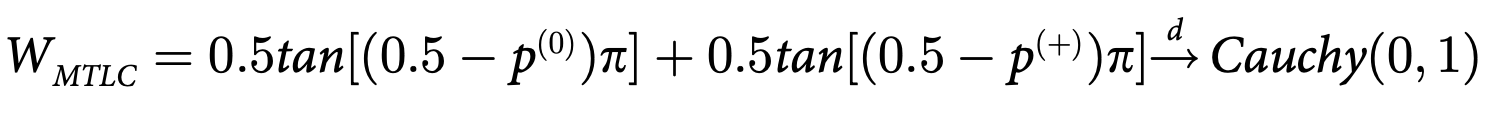
\includegraphics[width = \textwidth]{cauchy.png}
  \end{itemize}

\end{frame}
%--- Next Frame ---%

\begin{frame}[t]{Estimating correlation coefficients }
  \begin{itemize}
    \item Estimated values of correlation coefficients $\hat{\boldsymbol\rho}^{(0)}$ and $\hat{\boldsymbol\rho}^{(+)}$ may be different.
    \item When Pearson correlations are available to compute, the GEE estimates are similar.
  \end{itemize}
\end{frame}
%--- Next Frame ---%





\begin{frame}[t]{Discussion}
  \begin{itemize}
    \item MTLC accounts for taxonomic correlation structure and longitudinal correlation structure 
    \item MTLC has accurate Type I error, unbiased estimation of model parameters and robust power performance
    \item Correlation estimation is consistent
    \item Does not put a constraint on range of correlation coefficient
    \item Recommend using a subset of OTUs as model is time consuming when $N > 1000$.
  \end{itemize}
\end{frame}
%--- Next Frame ---%

\begin{frame}[t]{Thank you!}

\end{frame}
%--- Next Frame ---%

%------------------------------------------------

\begin{frame}
\frametitle{References}
\footnotesize{
\begin{thebibliography}{99} % Beamer does not support BibTeX so references must be inserted manually as below
\bibitem[Chen, 2020]{p1} Chen B, Xu W (2020)
\newblock Generalized estimating equation modeling on correlated microbiome sequencing data with longitudinal measures
\newblock \emph{PLoS Comput Biol } 16(9): e1008108. https://doi.org/10.1371/journal.pcbi.1008108.
\end{thebibliography}
}
\end{frame}

%------------------------------------------------


%----------------------------------------------------------------------------------------

\end{document}
